\chapter{Deployment}

\section{Introduction}
This section looks to explore some of the intricacies of the deployment process and certain elements of significance throughout, such as the use of the Composer PHP package manager, Bash scripting, and how to generate docblock documentation from PHPDoc in the Railrota source code.

\section{Composer}
Composer is a PHP package and dependency manager that is responsible for installing the required libraries and components that are specified within a \texttt{composer.json} file, and is also responsible for generating PSR-4 autoloaders on behalf of Laravel. \cite{Composer1} \cite{PSR1}

Composer is necessary for installing Railrota, or any Laravel application, and must be installed as part of the deployment process, either globally or used locally within the directory.

\section{Laravel Mix}
Laravel Mix, as mentioned in Chapter 5, is an implementation of Webpack for compiling front-end assets, and requires Node.js to run. It is not necessarily required on the server environment, as assets can be compiled in a development environment that does feature Node.js, before being uploaded to a server. \cite{Laravel2}

\section{Deployment Process}

\begin{figure}[!ht]
    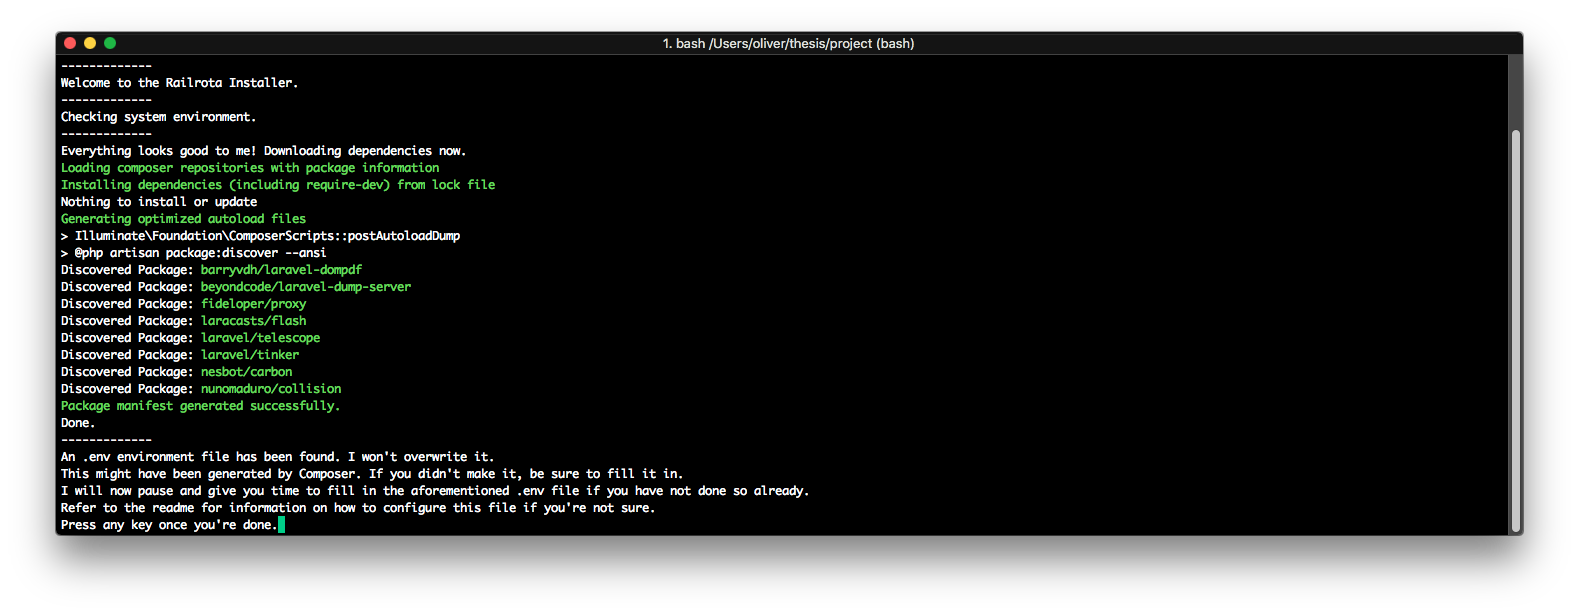
\includegraphics[width=\textwidth]{Figures/installer}
    \caption{Railrota installer currently running in a Bash terminal; invoking Composer and Laravel where necessary.}
    \label{fig:installer}
\end{figure}

\subsection{Deployment Script}
A script written in Bash, \texttt{install.sh}, has been written to help automate the installation process, that will take care of ensuring the necessary programming language prerequisites are met, that Composer is installed (or will retrieve a copy of it if not available), and for invoking the appropriate tools for installing Railrota in full. It will also attempt to invoke Laravel Mix to compile front-end assets, but will bypass this if Node.js and / or a suitable JavaScript package manager, either NPM or Yarn, are not installed.

Full information on this script is available in the project \texttt{readme.md} Markdown file, or in Appendix \ref{Project Readme}.

\subsection{Manual Deployment}
Full instructions on how to manually deploy Railrota can be found in the project \texttt{readme.md} Markdown file or in Appendix \ref{Project Readme}, though it can be safely assumed that any prior experience in installing Laravel 5.x applications is more than sufficient, as the process is does not significantly deviate as such.

\subsection{Generating Documentation}
PHPDoc is a code commenting convention commonly used in PHP applications, and is comparable to implementations such as JavaDoc in the Java language. It has been proposed as a working standard, but as of this time of writing remains unfinalised. \cite{PSR2} \cite{Joomla1}

Full HTML-based documentation can be generated from these code comments using Sami, a discontinued (but nevertheless functional) API documentation generator written itself in PHP. Information on how to run Sami and produce a \textit{docs} directory can be founded in the \texttt{readme.md} Markdown file or in Appendix \ref{Project Readme}. The standalone tool is included in the repository and is not a library or framework. \cite{Sami1}